\documentclass[aspectratio=169,11pt,hyperref={colorlinks=true}]{beamer}
\usepackage[utf8]{inputenc}
\usepackage[T1]{fontenc}
\usepackage{fontspec}
\usepackage[absolute,overlay]{textpos}
\usepackage{listingsutf8}
\usepackage{listings-golang}
\usepackage{tikz}
\usepackage{color}

\title{An intro to ko, developing the knative way}
\date[KubeCon NA]{Dec 12th 2018, Seattle, KubeCon NA}
\author[Andrea]{
  Andrea Frittoli \\
  Developer Advocate \\
  andrea.frittoli@uk.ibm.com \\
  @blackchip76
}

\usetheme{ibmcloud}

% Code style
\setlststyle

\lstdefinelanguage{koyaml}{
  keywords={github, com, afrittoli, examples, ms, go, helloworld},
  sensitive=false,
  comment=[l]{\#},
  morestring=[b]',
  morestring=[b]"
}

% Automatic section frame
\AtBeginSection{\frame{\sectionpage}}

\begin{document}

\begin{frame}[noframenumbering]
\titlepage{}
\end{frame}

\section{Microservice(s) in Go}

\begin{lgrayrwhiteframe}
  \frametitle{From local...}
  \large
  \begin{itemize}
    \item A few lines of code
    \item Build and run locally
    \item \small\texttt{github.com/afrittoli/examples/} \\
    \texttt{ms/go/helloworld}
  \end{itemize}
  \begin{textblock*}{0.4\paperwidth}(0.55\paperwidth,0cm)
    \begin{beamercolorbox}[leftskip=1cm,rightskip=1cm,rounded=true,sep=2.5ex]{Theorem}
        \lstinputlisting[language=Golang]{code/helloworld_ms.go}
    \end{beamercolorbox}
    \begin{beamercolorbox}[leftskip=1cm,rightskip=1cm,rounded=true]{Theorem}
        \lstinputlisting[language=bash]{code/build_and_run.sh}
    \end{beamercolorbox}
  \end{textblock*}
\end{lgrayrwhiteframe}

\begin{lblackrwhiteframe}
  \frametitle{...to the Cloud}
  \large
  \begin{beamercolorbox}[wd=0.3\paperwidth]{text}
    \begin{itemize}
      \item Scaling
      \item Resiliency
      \item Security
    \end{itemize}
  \end{beamercolorbox}%
  \begin{textblock*}{0.5\paperwidth}(0.5\paperwidth,0.2\paperheight)
    \centering
    
\includegraphics[width=0.20\paperwidth]{img/kubernetes.png}
    
\includegraphics[width=0.20\paperwidth]{img/istio.png}
    
\includegraphics[width=0.20\paperwidth]{img/knative.png}
  \end{textblock*}
\end{lblackrwhiteframe}

\begin{blackframe}
  \frametitle{Something is missing}
  \begin{textblock*}{\paperwidth}(0cm,0.2\paperheight)
    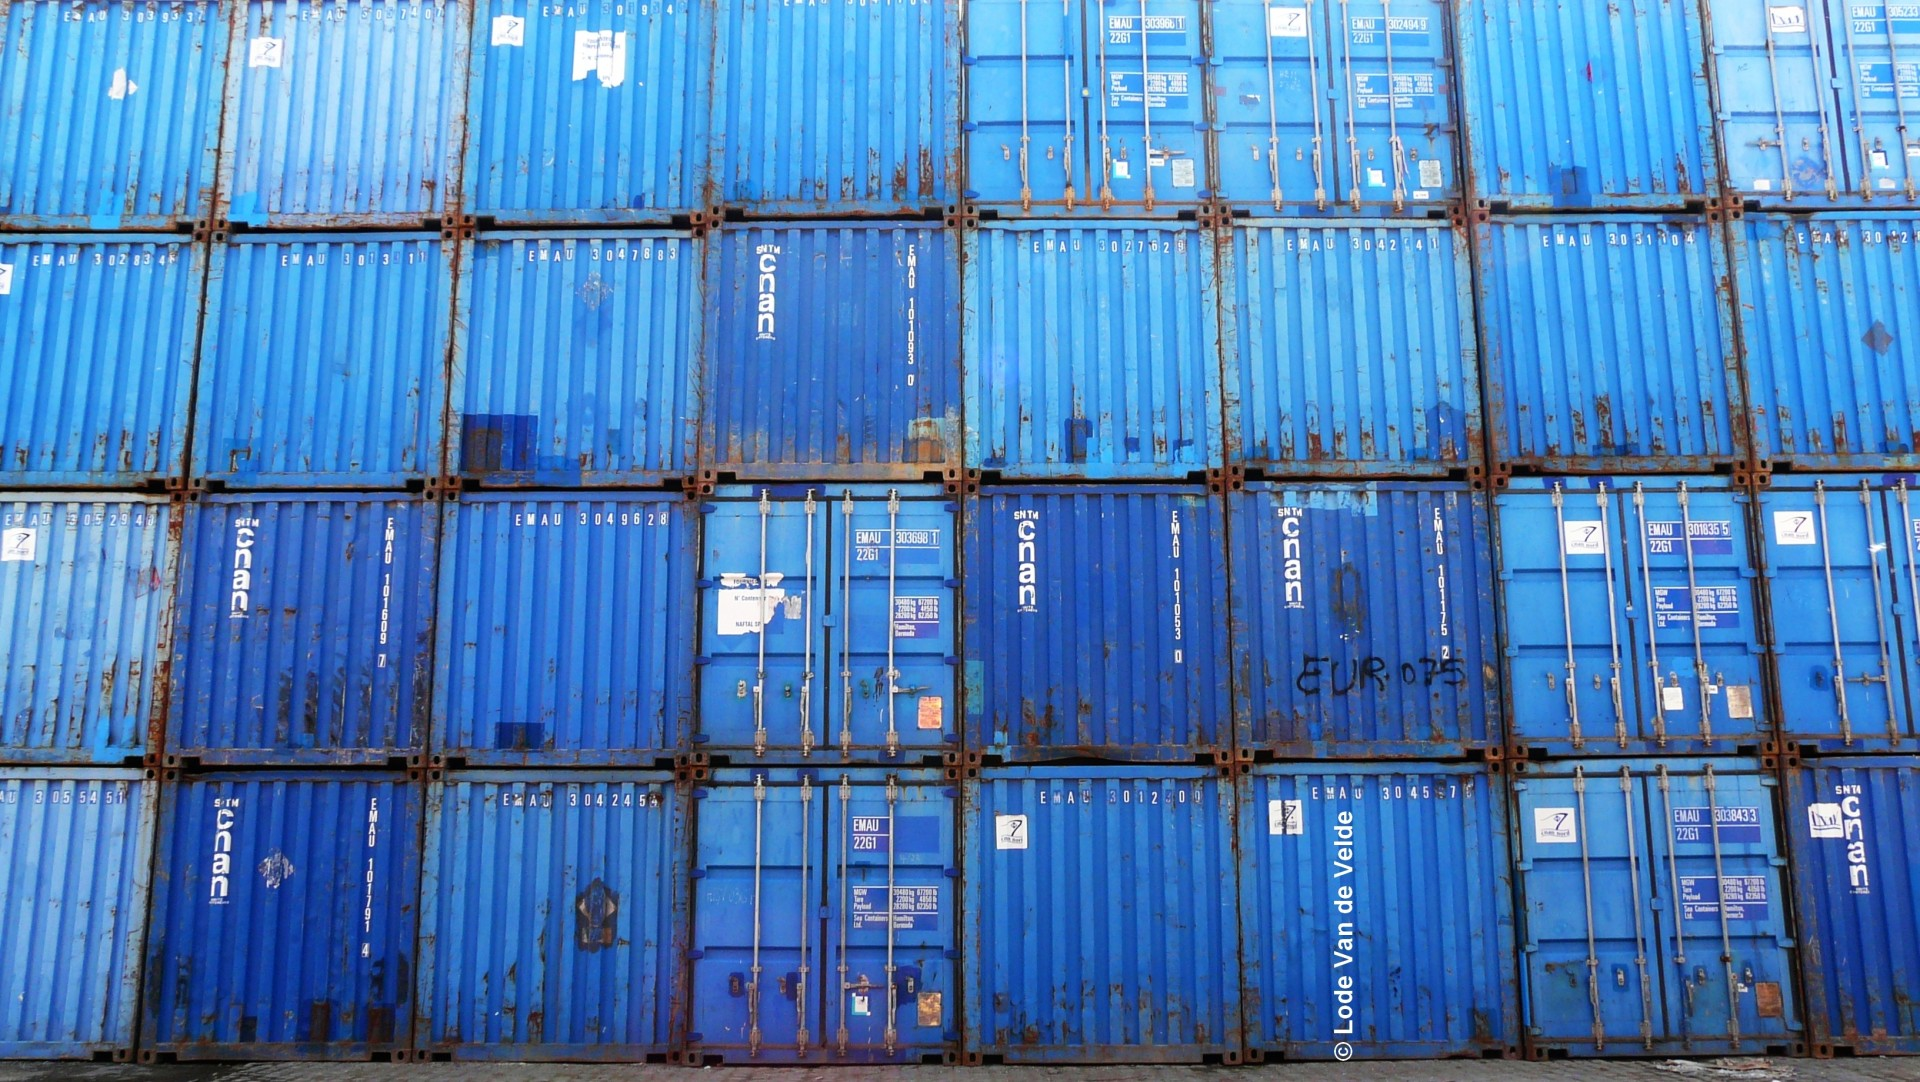
\includegraphics[width=\paperwidth]{img/blue-containers.jpg}
    % https://www.publicdomainpictures.net/pictures/100000/velka/blue-containers.jpg
  \end{textblock*}
  \begin{textblock*}{0.2\paperwidth}(0.83\paperwidth,0.93\paperheight)
    
\includegraphics[width=0.03\paperwidth]{img/cc.png}
    
\includegraphics[width=0.03\paperwidth]{img/zero.png}
  \end{textblock*}
\end{blackframe}

\begin{stripedframe}%
  {
    Containers!
    \begin{itemize}
      \item One to compile
      \item One to run
      \item A single Dockerfile for both
    \end{itemize}
  }%
  {
    \vspace{30pt}
    \setlststyledark
    \lstinputlisting[language=Docker]{code/Dockerfile}
    \setlststyle
  }%
  {
    Build the image \\
    Tag the image \\
    Push the image to the registry \\
    Update the image version \\
    \begin{itemize}
      \item Kubernetes manifests
      \item Helm chart values
    \end{itemize}
  }%
  {
    \vspace{30pt}
    \setlststyledark
    \lstinputlisting[language=bash]{code/docker_build_tag_push.sh}
    \setlststyle
  }%
\end{stripedframe}

\section{Getting Started with Ko}

\begin{tblackbgrayframe}
  \lstset{
    otherkeywords={*,...,/,.},
  }
  \frametitle{Invisible containers}
  \begin{textblock*}{\paperwidth}(0.32cm,0.2\paperheight)
    \lstinputlisting[language=koyaml]{code/deployment.yaml}
  \end{textblock*}
  \setlststyle
\end{tblackbgrayframe}

\begin{2columnsframe}%
  {
    Install {\color{ibmblue}\texttt{go}} \\
    and setup your environment: \\
    \vspace{1ex}
    \lstinputlisting[language=bash]{code/go.env}
    \vspace{3ex}
    Install {\color{ibmblue}\texttt{ko}}:
    \vspace{1ex}
    \lstinputlisting[language=bash]{code/install_ko.sh}
  }%
  {
    Congratulations! \\
    Ko is now available:
    \vspace{1ex}
    \lstinputlisting[language=bash]{code/ko_verify.sh}
  }
  \frametitle{Installing}
\end{grayframe}

\begin{2columnsframe}%
  {
    Import paths are hashed by default: \\
    \vspace{3ex}
    \tiny
    \texttt{%
      {\color{ibmdarkteal}github.com/afrittoli/examples/ms/go/}%
      {\color{ibmblue}helloworld}
    } \\
    $\Longrightarrow$ \texttt{%
      \$KO\_DOCKER\_REPO/{\color{ibmblue}helloworld}%
      -{\color{ibmdarkteal}<path-hash>}
    } \\
    \vspace{10ex}
    \normalsize
    Import paths can be preserved \\
    as long as the registry supports it: \\
    \vspace{3ex}
    \tiny
    \texttt{%
      {\color{ibmdarkteal}github.com/afrittoli/examples/ms/go/}%
      {\color{ibmblue}helloworld}
    } \\
    $\Longrightarrow$ \texttt{%
      \$KO\_DOCKER\_REPO/%
      {\color{ibmdarkteal}github.com/afrittoli/examples/ms/ \\
      go/}{\color{ibmblue}helloworld}
    } \\
  }%
  {
    Ko can use different container registries.\\
    \vspace{1ex}
    Using IBM Cloud Container Registry:
    \lstinputlisting[language=bash]{code/ibm_cr_auth_ko.sh}
  }
  \frametitle{Container Registry}
\end{2columnsframe}

\section{Publish, Resolve, Apply, Delete}

\begin{grayframe}
  \frametitle{Publish}
\end{grayframe}

\begin{grayframe}
  \frametitle{Resolve}
\end{grayframe}

\begin{grayframe}
  \frametitle{Apply \& Delete}
\end{grayframe}

\section{Ko and Knative}

\begin{grayframe}
  \frametitle{Developing Knative}
\end{grayframe}

\begin{grayframe}
  \frametitle{Knative \& Ko}
\end{grayframe}

\section{Q\&A}

\begin{blackframe}
  \frametitle{Thank You! Questions?}
  \vspace{30pt}
  \footnotesize\insertauthor\par---\par%
\end{blackframe}

\end{document}
